%----------------------------------------------------------------------------------------
%	PACKAGES AND OTHER DOCUMENT CONFIGURATIONS
%----------------------------------------------------------------------------------------

\documentclass{article}

\usepackage{fancyhdr} % Required for custom headers
\usepackage{lastpage} % Required to determine the last page for the footer
\usepackage{extramarks} % Required for headers and footers
\usepackage[usenames,dvipsnames]{color} % Required for custom colors
\usepackage{graphicx} % Required to insert images
\usepackage{listings} % Required for insertion of code
\usepackage{courier} % Required for the courier font
\usepackage{lipsum} % Used for inserting dummy 'Lorem ipsum' text into the template
\usepackage{epstopdf}
\usepackage{fancyhdr}
\usepackage{combelow}
\usepackage{enumerate}
\usepackage{amssymb,amsmath}
\usepackage{moreverb}
\usepackage{listings}
\usepackage{multirow}
\usepackage{verbatim}
\usepackage{epsfig}
\usepackage{epstopdf}
\usepackage{tabularx}
\usepackage{color}
\usepackage{subcaption}
\usepackage{tabulary}
\usepackage{algorithm2e}
\usepackage{wrapfig}
\usepackage{hyperref}
\usepackage[utf8]{inputenc}
\usepackage[table]{xcolor}
\usepackage{enumitem}

% Margins
\topmargin=-0.45in
\evensidemargin=0in
\oddsidemargin=0in
\textwidth=6.5in
\textheight=9.0in
\headsep=0.25in
\headheight=33pt

\linespread{1} % Line spacing

% Set up the header and footer
\pagestyle{fancyplain}
\fancyhf{}
\lhead{\MNTitle} % Top left header
%\chead{\MNTitleShort} % Top center head
\rhead{
\includegraphics[width=2cm]{Logo}} % Top right header
\lfoot{\MNClass} % Bottom left footer
\cfoot{} % Bottom center footer
\rfoot{Pagina\ \thepage\ din\ \protect\pageref{LastPage}} % Bottom right footer
\renewcommand\headrulewidth{0.4pt} % Size of the header rule
\renewcommand\footrulewidth{0.4pt} % Size of the footer rule

%----------------------------------------------------------------------------------------
%	CODE INCLUSION CONFIGURATION
%----------------------------------------------------------------------------------------

\definecolor{mygreen}{rgb}{0,0.6,0}
\definecolor{mygray}{rgb}{0.5,0.5,0.5}
\definecolor{mymauve}{rgb}{0.58,0,0.82}

\lstset{ %
  backgroundcolor=\color{white},		% choose the background color; you must add \usepackage{color} or \usepackage{xcolor}
  basicstyle=\small\ttfamily,		% the size of the fonts that are used for the code
  breakatwhitespace=false,			% sets if automatic breaks should only happen at whitespace
  breaklines=true,					% sets automatic line breaking
  captionpos=b,						% sets the caption-position to bottom
  commentstyle=\color{mygreen},		% comment style
  deletekeywords={...},				% if you want to delete keywords from the given language
  escapeinside={\%*}{*)},			% if you want to add LaTeX within your code
  extendedchars=true,				% lets you use non-ASCII characters; for 8-bits encodings only, does not work with UTF-8
  frame=single,						% adds a frame around the code
  keepspaces=true,					% keeps spaces in text, useful for keeping indentation of code (possibly needs columns=flexible)
  keywordstyle=\color{black},			% keyword style
  language=Octave,					% the language of the code
  morekeywords={*,...},				% if you want to add more keywords to the set
  numbers=left,						% where to put the line-numbers; possible values are (none, left, right)
  numbersep=6pt,						% how far the line-numbers are from the code
  numberstyle=\tiny\color{mygray},	% the style that is used for the line-numbers
  rulecolor=\color{black},			% if not set, the frame-color may be changed on line-breaks within not-black text (e.g. comments (green here))
  showspaces=false,					% show spaces everywhere adding particular underscores; it overrides 'showstringspaces'
  showstringspaces=false,			% underline spaces within strings only
  showtabs=false,					% show tabs within strings adding particular underscores
  stepnumber=1,						% the step between two line-numbers. If it's 1, each line will be numbered
  stringstyle=\color{mymauve},		% string literal style
  tabsize=2,							% sets default tabsize to 2 spaces
  title=\lstname						% show the filename of files included with \lstinputlisting; also try caption instead of title
}

% Creates a new command to include a perl script, the first parameter is the filename of the script (without .pl), the second parameter is the caption
\newcommand{\octavescript}[2]{
\begin{itemize}
\item[]\lstinputlisting[caption=#2,label=#1]{#1.m}
\end{itemize}
}

%----------------------------------------------------------------------------------------
%	DOCUMENT STRUCTURE COMMANDS
%	Skip this unless you know what you're doing
%----------------------------------------------------------------------------------------

\setcounter{secnumdepth}{0} % Removes default section numbers
\newcounter{ProblemCounter} % Creates a counter to keep track of the number of problems

\newcommand{\ProblemName}{}
\newenvironment{Problem}[1][Sectiunea \arabic{ProblemCounter}]{ % Makes a new environment called Problem which takes 1 argument (custom name) but the default is "Problem #"
\stepcounter{ProblemCounter} % Increase counter for number of problems
\renewcommand{\ProblemName}{#1} % Assign \ProblemName the name of the problem
\section{\ProblemName} % Make a section in the document with the custom problem count
}{}

\newcommand{\ProblemAnswer}[1]{ % Defines the problem answer command with the content as the only argument
\noindent\framebox[\columnwidth][c]{\begin{minipage}{0.98\columnwidth}#1\end{minipage}} % Makes the box around the problem answer and puts the content inside
}

\newcommand{\SectionName}{}
\newenvironment{Section}[1]{ % New environment for sections within  problems, takes 1 argument - the name of the section
\renewcommand{\SectionName}{#1} % Assign \SectionName to the name of the section from the environment argument
\subsection{\SectionName} % Make a subsection with the custom name of the subsection
}{}

%----------------------------------------------------------------------------------------
%	NAME AND CLASS SECTION
%----------------------------------------------------------------------------------------

\newcommand{\MNTitle}{Tema\ \#1 Game of Life} % Assignment title
\newcommand{\MNDueDate}{17-Apr-2022 23:55} % Due date
\newcommand{\MNClass}{SISTEME TOLERANTE LA DEFECTE} % Course/class
\newcommand{\MNClassTime}{} % Class/lecture time

%----------------------------------------------------------------------------------------
%	TITLE PAGE
%----------------------------------------------------------------------------------------

\title{
%\vspace{2in}
\textmd{\textbf{\MNClass \\ \MNTitle}}\\
\normalsize\vspace{0.1in}\small{Termen de predare: \MNDueDate}\\
}

\date{} % Insert date here if you want it to appear below your name

%----------------------------------------------------------------------------------------

\begin{document}

\maketitle

%----------------------------------------------------------------------------------------
%    TABLE OF CONTENTS
%----------------------------------------------------------------------------------------

%\setcounter{tocdepth}{1} % Uncomment this line if you don't want subsections listed in the ToC

%\newpage
%\tableofcontents
%\newpage


%----------------------------------------------------------------------------------------
%    OBIECTIVELE TEMEI DE CASA
%----------------------------------------------------------------------------------------
\section{Obiective}

Scopul acestei teme este de a implementa, în C, folosind biblioteca MPI, un program distribuit, scalabil cu numărul de procese, având ca scop simularea jocului Game of Life - B3/S23 introdus de John Conway.

%----------------------------------------------------------------------------------------
%    PROBLEM 1
%----------------------------------------------------------------------------------------

% To have just one problem per page, simply put a \clearpage after each problem

\begin{Problem}[Date introductive]

Jocul presupune existența unei hărți sub forma unei matrici de dimensiune H x W. Fiecare element având una din următoarele două valori:

\begin{itemize}
 - \textbf{Individ}, valoarea \textbf{1}\newline
 - \textbf{Gol}, valoarea \textbf{0}
\end{itemize}


Simularea va fi executată pentru un număr dat de etape. În fiecare etapă elementele din matrice își schimbă valoarea după setul de reguli B3/S23:
\begin{enumerate}[label=(\alph*)]
    \item Un individ nou este creat dacă are 3 vecini;
    \item Un individ continuă să existe dacă are 2 sau 3 vecini;
    \item Orice individ cu 1, 0 sau mai mult de 3 vecini dispare.
\end{enumerate}

Vecinii unui element sunt cele 8 căsuțe reprezentate în tabelul \ref{tab:map} cu verde.

\begin{table}[!hb]
    \centering
    \caption{Exemplu hartă, vecini}
    \begin{tabular}{ | m{0.5cm} | m{0.5cm}| m{0.5cm} | m{0.5cm} |m{0.5cm} | } 
      \hline
      & & & & \\ 
      \hline
      & \cellcolor{green!25} & \cellcolor{green!25} &\cellcolor{green!25} & \\ 
      \hline
      & \cellcolor{green!25}& & \cellcolor{green!25}& \\ 
      \hline
      & \cellcolor{green!25} & \cellcolor{green!25} &\cellcolor{green!25} & \\
      \hline
      & & & & \\ 
      \hline
    \end{tabular}
    \label{tab:map}
\end{table}

\clearpage
\end{Problem}

\section{ }

\begin{Problem}[Reprezentare hartă]

\newline \newline Există două metode de a reprezenta harta:   
\begin{enumerate}[label=(\alph*)]
    \item Ca un plan, marginile vor fi alcătuite (tot timpul) din elemente goale; 
    \item Ca un toroid: astfel, prima linie/coloană este lipită de ultima. Deci, zona simulată nu va conține margini.
\end{enumerate}

\begin{table}[!hbt]
    \begin{minipage}{.5\linewidth}
      \centering
        \caption{Plan}
        \begin{tabular}{ | m{0.5cm} | m{0.5cm}| m{0.5cm} | m{0.5cm} | m{0.5cm} | m{0.5cm} | }
          \hline
          \rowcolor{lightgray}
          0 & 0 & 0 & 0 & 0 & 0\\ 
          \hline
          \cellcolor{lightgray} 0 & A & B & C & D & \cellcolor{lightgray} 0\\ 
          \hline
          \cellcolor{lightgray} 0 & E & F & G & H & \cellcolor{lightgray} 0\\ 
          \hline
          \cellcolor{lightgray} 0 & I & J & K & L & \cellcolor{lightgray} 0\\ 
          \hline
          \rowcolor{lightgray}
          0 & 0 & 0 & 0 & 0 & 0\\ 
          \hline
        \end{tabular}
    \end{minipage} 
    \begin{minipage}{.5\linewidth}
        \caption{Toroid}
        \centering
        \begin{tabular}{ | m{0.5cm} | m{0.5cm}| m{0.5cm} | m{0.5cm} | m{0.5cm} | m{0.5cm} | } 
          \hline
          \rowcolor{lightgray}
          L & I & J & K & L & I\\ 
          \hline
          \cellcolor{lightgray} D & A & B & C & D & \cellcolor{lightgray} A\\ 
          \hline
          \cellcolor{lightgray} H & E & F & G & H & \cellcolor{lightgray} E\\ 
          \hline
          \cellcolor{lightgray} L & I & J & K & L & \cellcolor{lightgray} I\\ 
          \hline
          \rowcolor{lightgray}
          D & A & B & C & D & A\\ 
          \hline
        \end{tabular}
    \end{minipage}
\end{table}

\end{Problem}

\begin{Problem}[Procesul de simulare]

Simularea va fi constituită dintr-un număr de etape, starea celulelor schimbându-se simultan în funcție de celulele din etapa anterioară.


Programul va primi ca input un fișier și un număr de pași care va reprezenta numărul de etape ale simulării, iar rezultatul final va fi scris într-un fișier de ieșire.

\begin{figure}[!hb]
    \begin{center}Exemplu simulare pe o hartă de dimensiune 6 x 5\end{center}
    \centering
    \begin{subfigure}[b]{0.3\textwidth}
        \centering
        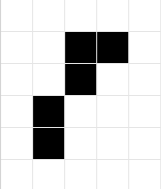
\includegraphics[width=3cm]{simulation_4x5_0.png}
        \caption{Harta inițială}
    \end{subfigure}
    \begin{subfigure}[b]{0.3\textwidth}
        \centering
        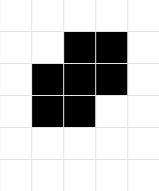
\includegraphics[width=3cm]{simulation_4x5_1.png}
        \caption{După pasul 1}
    \end{subfigure}
    \begin{subfigure}[b]{0.3\textwidth}
        \centering
        
\includegraphics[width=3cm]{simulation_4x5_2.png}
        \caption{După pasul 2}
    \end{subfigure}
\end{figure}

\end{Problem}

\clearpage

\section {}

\begin{Problem}[Rularea programului]

Rularea programului se va realiza astfel:\\

\begin{lstlisting}
mpirun --oversubscribe -np NUM_PROCS ./homework IN_FILENAME OUT_FILENAME NUM_STEPS
\end{lstlisting}

Unde:

\begin{itemize}
    \item \textbf{NUM\textunderscore PROCS} - numărul de procese;
    \item \textbf{IN\textunderscore FILENAME} - numele (path-ul) fișierului de intrare;
    \item \textbf{OUT\textunderscore FILENAME} - numele (path-ul) fișierului de ieșire;
    \item \textbf{NUM\textunderscore STEPS} - numărul de pași ai simulării.
\end{itemize}

Exemplu:
\begin{lstlisting}
mpirun --oversubscribe -np 2 ./homework in1.txt out1.txt 567
\end{lstlisting}

\end{Problem}

\begin{Problem}[Fișiere de intrare/ieșire]

Pe prima linie vom avea:
\begin{itemize}
    \item O literă P (plan) sau T (toroid) ce indică tipul hărții;
    \item Un număr întreg H ce indică lățimea hărții;
    \item Un număr întreg W ce indică lungimea hărții;
    \item H linii cu W valori, pentru fiecare celulă din hartă (1 - individ, 0 - gol).
\end{itemize}
Exemplu: \\

\begin{table}[!hb]
    \centering
\end{table}

\begin{table}[!hbt]
    \begin{minipage}{.5\linewidth}
      \centering
        \caption{Exemplu fișier de intrare}
        \begin{tabular}{ m{0.5cm} m{0.5cm} m{0.5cm} m{0.5cm} } 
          P & 5 & 4\\
          0 & 1 & 1 & 0\\ 
          0 & 1 & 0 & 0\\ 
          1 & 0 & 0 & 0 \\ 
          1 & 0 & 0 & 0 \\
          0 & 0 & 0 & 0 \\      
        \end{tabular}
    \end{minipage} 
    \begin{minipage}{.5\linewidth}
        \centering
        \caption{Exemplu fișier de ieșire}
        \begin{tabular}{ m{0.5cm} m{0.5cm} m{0.5cm} m{0.5cm} } 
          P & 5 & 4\\
          0 & 1 & 1 & 0\\ 
          1 & 1 & 1 & 0\\ 
          1 & 1 & 0 & 0 \\ 
          0 & 0 & 0 & 0 \\
          0 & 0 & 0 & 0 \\      
        \end{tabular}
    \end{minipage}
\end{table}

\end{Problem}

\section {}

\begin{Problem}[Trimitere și punctare]

\begin{itemize}
    \item Este necesară crearea unei arhive \textbf{.zip} care trebuie să conțină fișierul ``homework.c'' și uploadarea acesteia în cadrul checker-ului.
    \item O temă care nu compilează va primi 0 puncte. Tema va fi rulată și testată pentru corectitudine și scalabilitate pe un checker al ATM.
    \item Link-ul către acest checker va fi transmis ulterior.\\
\end{itemize}

\textbf{Orice încercare de a abuza checker-ul va duce la un punctaj de 0 pe toate temele.} \\

Distribuția punctajului este următoarea:
\begin{itemize}
    \item 70 puncte - Output corect program distribuit și scalabil pentru hărți de tipul PLAN.
    \item 30 puncte - Output corect program distribuit și scalabil pentru hărți de tipul TOROID.
\end{itemize}

Arhiva .zip trebuie să conțină fișierele ``homework.c''. O temă care nu compilează va primi 0 puncte. Tema va fi rulată și testată pentru corectitudine și scalabilitate pe un checker al ATM. Link-ul către acest checker va fi transmis ulterior.

\textbf{Orice încercare de a abuza checker-ul va duce la un punctaj de 0 pe toate temele.}

\end{Problem}

\end{document}